%
% Cifrados de flujo.
% Proyecto Lovelace.
%

\newpage
\section{Cifrados de flujo}

A diferencia de los cifrados de bloque, que trabajan sobre grupos enteros de
bits a la vez, los cifrados de flujo trabajan sobre bits individuales,
cifrándolos uno por uno. Una manera de verlos es como cifrados por bloques con
un tamaño de bloque igual a 1.

Un cifrado de flujo aplica transformaciones de acuerdo a un flujo de llave:
una secuencia de símbolos pertenecientes al espacio de llaves. El flujo de
llave puede ser generado de manera aleatoria, o por un algoritmo
pseudoaleatorio que toma una semilla a la entrada, o por una semilla y
símbolos cifrados anteriormente.

Entre las ventajas de los cifrados de flujo sobre los cifrados de bloque se
encuentran el hecho de que son más rápidos en hardware, son más útiles cuando
el buffer es limitado o se necesita procesar la información al momento de
llegada. La propagación de los errores es limitada o nula, por lo que también
son más útiles en casos en los que hay probabilidades altas de errores en la
transmisión \cite{menezes}.

Los cifrados de bloques funcionan sin ninguna clase de memoria (por sí solos);
en contraste, la función de cifrado de un cifrado de flujo puede variar
mientras se procesa el texto en claro, por lo cuál tienen un mecanismo de
memoria asociado. Otra denominación para estos cifrados es \textit{de estado},
por que la salida no depende solamente del texto en claro y de la llave, sino
que también depende del estado actual.

Una clasificación común es en \textit{síncronos} y
en \textit{autosincronizables}. A continuación describimos a grandes rasgos
ambos modelos.

\subsection{Síncronos}

Un cifrado de flujo síncrono es aquel en el que el flujo de la llave es
generado de manera independiente del texto en claro y del texto cifrado. Se
puede definir un modelo general con las siguientes tres ecuaciones.

\begin{equation}
  \label{cambio_de_estado}
  e_{i+1} = f(e_i, L)
\end{equation}

\begin{equation}
  \label{flujo_de_llave}
  l_i = g(e_i, L)
\end{equation}

\begin{equation}
  \label{funcion_de_salida}
  c_i = h(l_i, m_i)
\end{equation}

\vspace{0.5cm}

La letra $ e $ representa el estado del cifrado,$ L $ es la llave, $ l $ es
la salida del flujo de llave, $ c $ es el texto cifrado y $ m $ es el texto en
claro. La función de la ecuación \ref{cambio_de_estado} ($ f $) es la que
describe el cambio de estado; este se determina a partir del estado actual y
de la llave. En la ecuación \ref{flujo_de_llave} se describe la acción del
flujo de llave ($ g $): para determinar el próximo símbolo se emplea solamente
el estado actual y la llave. La tercera ecuación (\ref{funcion_de_salida},
$ h $) describe la acción de combinar el flujo de la llave con el mensaje, y
así obtener el texto cifrado.

% TODO: referencia a sección de OFB.

En la figura \ref{flujo_sincrono} se describe de manera gráfica las operaciones
de cifrado y descifrado; estas guardan muchas similitudes con el modo de
operación OFB, con la única excepción de que este trabaja con bloques del tamaño
del cifrado subyacente. En otras palabras, si definiéramos el tamaño del bloque
(y en consecuencia el tamaño del vector de inicialización) como 1, entonces
OFB sería un cifrado de flujo síncrono.

\vspace{0.5cm}

\begin{figure}[H]
  \centering
  \begin{subfigure}{0.45\textwidth}
    \begin{center}
      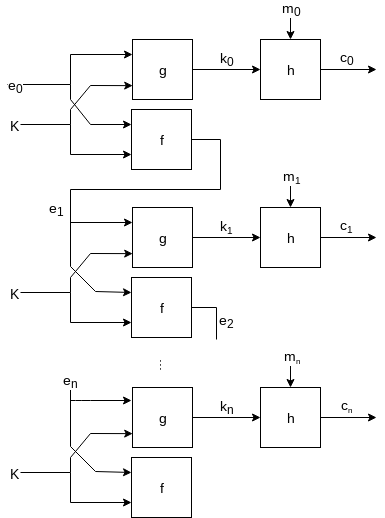
\includegraphics[width=0.9\linewidth]
        {contenidos/antecedentes/cifrados_de_flujo/diagramas/sincrono_cifrado.png}
      \caption{Cifrado.}
    \end{center}
  \end{subfigure}
  \begin{subfigure}{0.45\textwidth}
    \begin{center}
      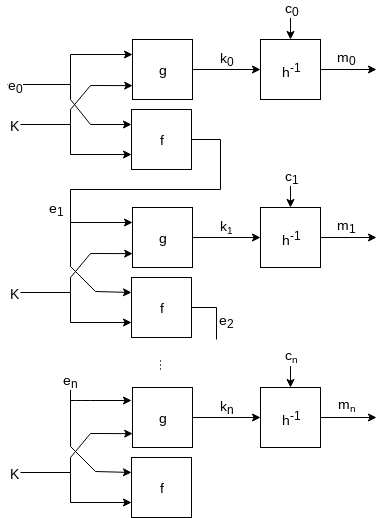
\includegraphics[width=0.9\linewidth]
        {contenidos/antecedentes/cifrados_de_flujo/diagramas/sincrono_descifrado.png}
      \caption{Descifrado.}
    \end{center}
  \end{subfigure}
  \caption{Esquema general de un cifrado de flujo síncrono.}
  \label{flujo_sincrono}
\end{figure}

\subsection{Autosincronizables}
